\input{../YKY-preamble.tex}
% \usepackage[no-math]{fontspec}
% \setmainfont[BoldFont=Alibaba_Sans_Regular.otf,ItalicFont=Alibaba_Sans_Light_Italic.otf]{Alibaba_Sans_Light.otf}

\usepackage[backend=biber]{biblatex}
\bibliography{../AGI-book}

\usepackage[active,tightpage]{preview}		% for continuous page(s)
\renewcommand{\PreviewBorder}{0.5cm}
\renewcommand{\thempfootnote}{\arabic{mpfootnote}}

\usepackage[absolute,overlay]{textpos}		% for page number on upper left corner

\usepackage{color}
% \usepackage{mathtools}
\usepackage[hyperfootnotes=false]{hyperref}

% \usepackage[backend=biber,style=numeric]{biblatex}
% \bibliography{../AGI-book}
% \renewcommand*{\bibfont}{\footnotesize}

\usetikzlibrary{shapes}
% \usepackage[export]{adjustbox}	% ??
\usepackage{verbatim} % for comments
% \usepackage{newtxtext,newtxmath}	% Times New Roman font

% \titleformat{\subsection}[hang]{\bfseries\large\color{blue}}{}{0pt}{} 
% \numberwithin{equation}{subsection}

\newcommand{\underdash}[1]{%
	\tikz[baseline=(toUnderline.base)]{
		\node[inner sep=1pt,outer sep=10pt] (toUnderline) {#1};
		\draw[dashed] ([yshift=-0pt]toUnderline.south west) -- ([yshift=-0pt]toUnderline.south east);
	}%
}%

\newcommand\reduline{\bgroup\markoverwith{\textcolor{red}{\rule[-0.5ex]{2pt}{0.4pt}}}\ULon}

%\DeclareSymbolFont{symbolsC}{U}{txsyc}{m}{n}
%\DeclareMathSymbol{\strictif}{\mathrel}{symbolsC}{74}
%\DeclareSymbolFont{AMSb}{U}{msb}{m}{n}
%\DeclareSymbolFontAlphabet{\mathbb}{AMSb}
%\setmathfont{lmroman17-regular.otf}
\DeclareMathOperator*{\argmin}{arg\,min}
\DeclareMathOperator*{\argmax}{arg\,max}

% \usepackage[most]{tcolorbox}
%\tcbset{on line, 
%	boxsep=4pt, left=0pt,right=0pt,top=0pt,bottom=0pt,
%	colframe=red,colback=pink,
%	highlight math style={enhanced}
%}
%\newcommand{\atom}{\vcenter{\hbox{\tcbox{....}}}}

\let\oldtextbf\textbf
\renewcommand{\textbf}[1]{\textcolor{blue}{\oldtextbf{#1}}}

\newcommand{\logic}[1]{{\color{violet}{\textit{#1}}}}
\newcommand{\underconst}{\includegraphics[scale=0.5]{../2020/UnderConst.png}}
\newcommand{\KBsymbol}{\vcenter{\hbox{\includegraphics[scale=1]{../KB-symbol.png}}}}
\newcommand{\token}{\vcenter{\hbox{\includegraphics[scale=1]{token.png}}}}
\newcommand{\proposition}{\vcenter{\hbox{\includegraphics[scale=0.8]{proposition.png}}}}

\begin{document}

\begin{preview}

\title{\vspace{-1.5cm} \bfseries\color{blue}{\LARGE Why I think reinforcement learning can solve the hallucination problem}}

% \author{YKY} % Your name
\date{\vspace{-2cm}} % Date, can be changed to a custom date

\maketitle

\setcounter{section}{-1}
\newcounter{mypage}
\setcounter{mypage}{1}

% (1) Circled page number on upper left corner
\begin{textblock*}{5cm}(2.1cm,2.3cm) % {block width} (coords) 
{\color{red}{\large \textcircled{\small \themypage}}}
\addtocounter{mypage}{1}
\end{textblock*}

\begin{minipage}{\textwidth}
\setlength{\parskip}{0.4\baselineskip}

The Transformer is an extremely \textbf{compressive} algorithm, due to its sharing the $Q,K,V$ matrices across every layer (though there may be 100's of layers):
\begin{equation}
	\vcenter{\hbox{
\includegraphics[scale=1]{Transformer-is-super-compressive.png}}}
\end{equation}
As a learning machine has only a finite number of weights (parameters), when it is ``forced'' to predict and re-construct the data, it must learn the abstract rules or patterns of the data.

\textbf{Occam's razor} is the idea that knowledge is acquired by finding the simplest explanations of the world (data).

Reinforcement learning is special in that it puts logic inference into a \textbf{closed loop}, ie, repeatedly iterating a \textbf{transition function}:
\begin{equation}
\vcenter{\hbox{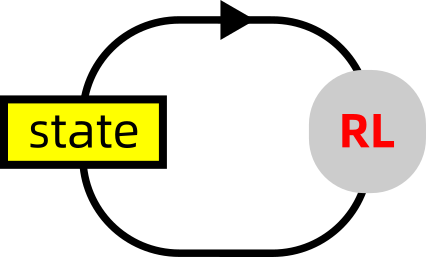
\includegraphics[scale=0.8]{minimal-RL.png}}}
\end{equation}
Under this setting, the transition function will be forced to explain the world with a compact set of rules, thus acquiring the knowledge / intelligence needed to discern truth from falsehood, thus solving the hallucination problem.

Indeed, the GPT / Transformer is already doing something like this, although it does not have an explicit closed-loop as in RL, it is still trained with an implicit loop over all data (the corpus).

My hope is for RL's closed loop to increase the \textbf{re-use} of logic rules, thus increasing the model's intelligence -- according to Occam's razor.

\end{minipage}
\end{preview}

\begin{preview}
\begin{textblock*}{5cm}(2.1cm,2.3cm) % {block width} (coords) 
	{\color{red}{\large \textcircled{\small \themypage}}}
	\addtocounter{mypage}{1}
\end{textblock*}

\begin{minipage}{\textwidth}
	\setlength{\parskip}{0.4\baselineskip}

\section{Two architectures}

Recall that the \textbf{Auto-Encoder} (AE) has the dual functions of \textbf{compression} and \textbf{predicting the future}, so we use this symbol for it:
\begin{equation}
\vcenter{\hbox{
\includegraphics[scale=1]{autoencoder-symbol.png}}}
\end{equation}

We can think of two architectures, based on how we interpret the functions of an Auto-Encoder.

\textbf{Architecture \#1}: AE emulates human thinking.
\begin{equation}
\vcenter{\hbox{
\includegraphics[scale=0.7]{AE-architecture-1.png}}}
\end{equation}
Thoughts = natural-language sentences.  \\
RL puts inference into a closed loop.  \\
Thoughts describe the world.

\textbf{Architecture \#2}: AE = compressed world model.
\begin{equation}
\vcenter{\hbox{
\includegraphics[scale=0.7]{AE-architecture-2.png}}}
\end{equation}
Thoughts = hidden / latent state.  \\
RL helps AE to explain the world, \\
successful explanations reward RL.

\subsection{Which architecture is correct?}

It may appear strange that AE has two different interpretations.  Because
\begin{equation}
\mbox{human thinking} \subset \mbox{world} ,
\end{equation}
we can see that human thinking, as appears in text corpuses, can sometimes be wrong due to eg. lying, false beliefs, etc.  Therefore Arch \#1 can be faulty and may be the origin of hallucinations.

%The actor and critic seem distinct from the world model.  The world model learns to predict the next state from the current state and action, ie. $p(s_{t+1} | s_t, a_t)$.  As such, it is not influenced by rewards or ``value judgements''.  We could say that the world model seeks only the ``\textbf{truth}'', whereas the actor-critic seeks values \footnote{but we can also let the world model predict rewards as well, in which case its role partly overlaps with the critic.}.  How might a world model help RL be more efficient?  Perhaps by letting the actor-critic explore the world model virtually:
%\begin{equation}
%	\vcenter{\hbox{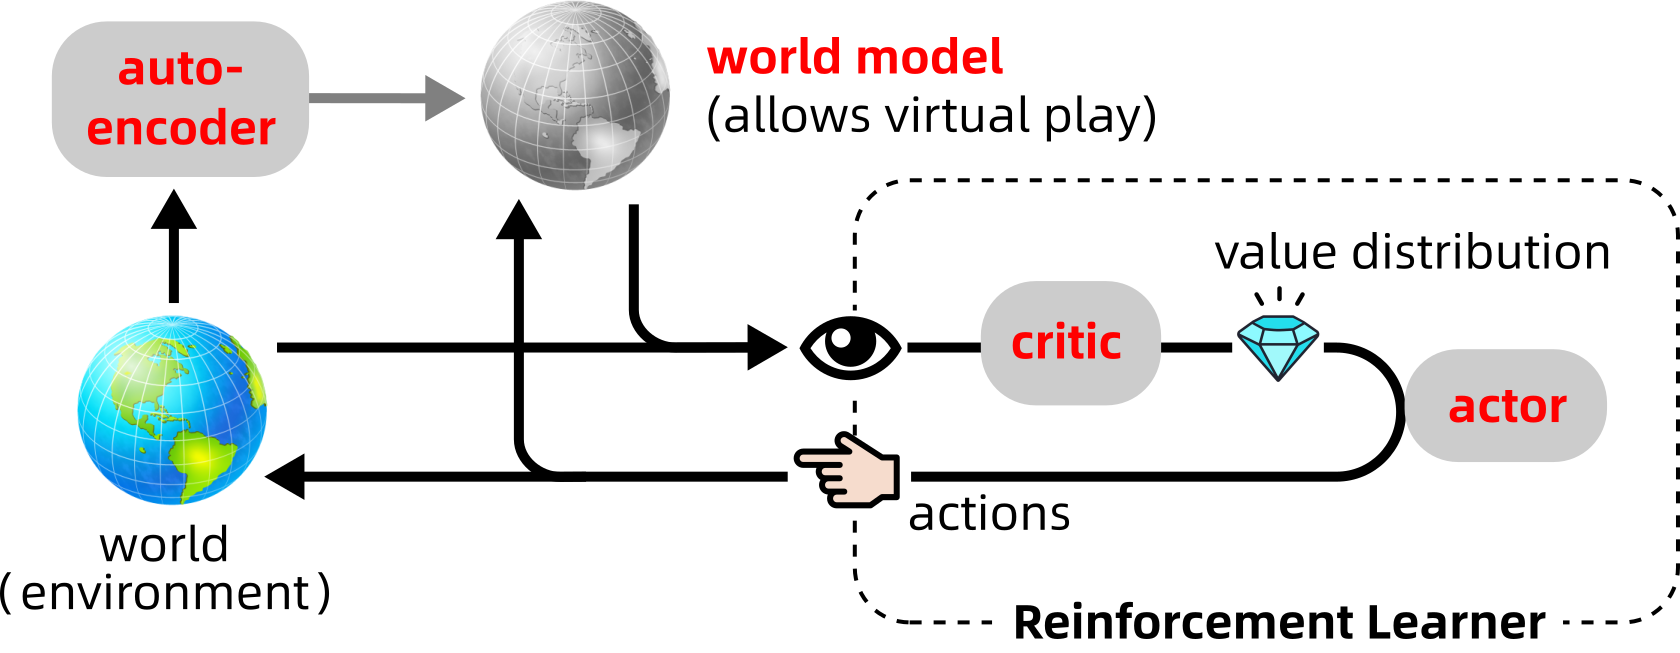
\includegraphics[scale=0.8]{RL-with-world-model.png}}}
%\end{equation}
%This is significant in physical environments, where physical actions are much more costly.  Ironically, most current AI training environments are already virtual, so this may not bring about large improvements.

\end{minipage}
\end{preview}

\begin{preview}
\begin{textblock*}{5cm}(2.1cm,2.3cm) % {block width} (coords) 
{\color{red}{\large \textcircled{\small \themypage}}}
\addtocounter{mypage}{1}
\end{textblock*}

\begin{minipage}{\textwidth}
\setlength{\parskip}{0.4\baselineskip}

\section{Iteration helps compression}

Consider the following simplified scenario:
\begin{equation}
\vcenter{\hbox{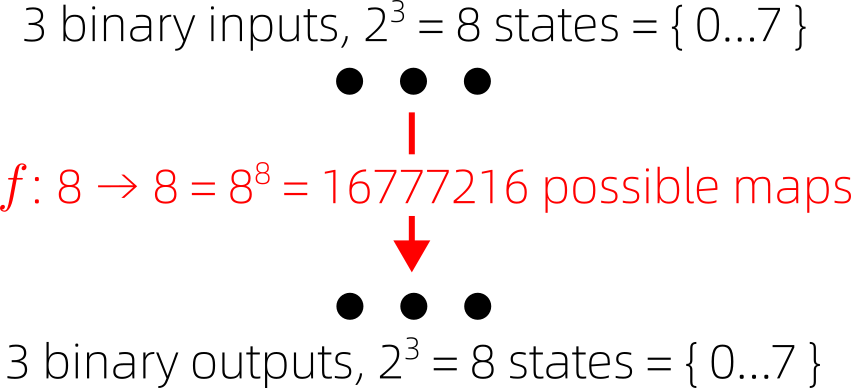
\includegraphics[scale=0.8]{iteration-more-mappings-1.png}}}
\end{equation}
If $f \in \mathcal{F} = 8^8$ then all possible mappings are learnable.  In general the family of $f$ may be a subset of all possible maps, as long as some solution(s) exist in $\mathcal{F}$.

What if $f$ is iterated?
\begin{equation}
\vcenter{\hbox{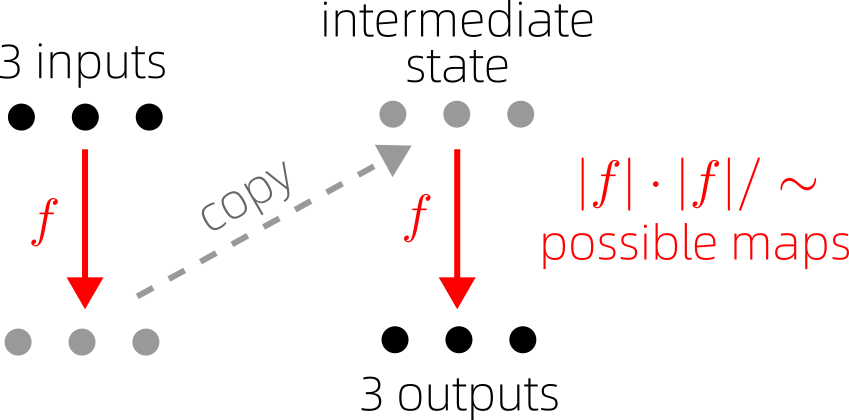
\includegraphics[scale=0.8]{iteration-more-mappings-2.png}}}
\end{equation}
Then the number of maps $f \circ f$ is $|f| \cdot |f|$ quotiented by redundancy.

In neural networks, $f \circ f$ is two neural networks \textbf{stacked} together.  It has \textbf{twice} the number of layers (and weights).  In general, the number of mappings of a neural network grows as the \textbf{exponent} of the number of layers\footnote{For an intuitive explanation, think of $f$ as a polynomial of degree $d$, then $f_1 \circ f_2$ has degree $d_1 \cdot d_2$.  The number of ``zero-crossings'' of a polynomial is same as its degree.  Thus in general a polynomial can ``cut'' the ambient space into $d$ pieces.}, which is consistent with $|f|\cdot|f|$.

In other words, the number of maps representable by a big neural network is the same as if the network is broken into smaller pieces, as long as the layers add up to the same number.  However, if the weights of each piece are \textbf{shared}, then it obviously results in more compact \textbf{information compression}, while training time $\propto$ number of weights which remains the same (shared weights counted with multiplicity).

\subsection{Conclusions}

\begin{itemize}
	\item \cc{
	有 loop 和没有 loop 的 \textbf{训练时间} 是差不多的,但其 \textbf{智能} 会提升。 
	}{
	If iterated, training time may be roughly the same, but intelligence would increase. }

	\item 中间状态的 语义是 \textbf{浮动} 的,只有通过训练才能确定。 因此,GPT 训练出来的权重 不能在这里 \textbf{再用},需要重新训练。

\end{itemize}

\end{minipage}
\end{preview}

\begin{preview}
\begin{textblock*}{5cm}(2.1cm,2.3cm) % {block width} (coords) 
	{\color{red}{\large \textcircled{\small \themypage}}}
	\addtocounter{mypage}{1}
\end{textblock*}

\begin{minipage}{\textwidth}
	\setlength{\parskip}{0.4\baselineskip}

\section{About our group}

We operate as a \textbf{DAO} (decentralized autonomous organization) based on transparent operations and reward system based on weighted voting, to enable global collaboration without racial (or other forms of) discrimination.

Our values:
\begin{itemize}
	\item democracy
	\item freedom of speech
	\item racial equality
	\item transparency
	\item tolerance of mistakes
	\item a learning environment
\end{itemize}

It is OK for anyone to challenge other member's theories, ideas, proposals, etc.

\end{minipage}
\end{preview}

\end{document}
